\chapter{Applications}
\label{chap:apps}

As mentioned in previous chapters, the SSaaS model can be utilized
across a range of applications. In each case, the model allows users
to reduce the trust they must place in any single third-party while
also supporting popular use cases. I present several potential SSaaS
applications in this chapter. Some of these applications are also
discussed in~\cite{custos-trios}.

\section{Storage}

One of the primary applications of the SSaaS model is to secure
storage systems, both local and hosted. These applications are all
variations on the previously discussed encrypted data + SSaaS-backed
keys model. In such applications, applications handle the encryption
and verification of data locally, sending only encrypted data to third
parities or storing such data on high risk devices. In order to ensure
that such client-side encryption does not break traditional features
associated with cloud and mobile data storage, clients store the
associated encryption keys with one or more Secret Storage Providers.

\subsection{Cloud File Sync/Storage}

\begin{figure}[t]
  \centering
  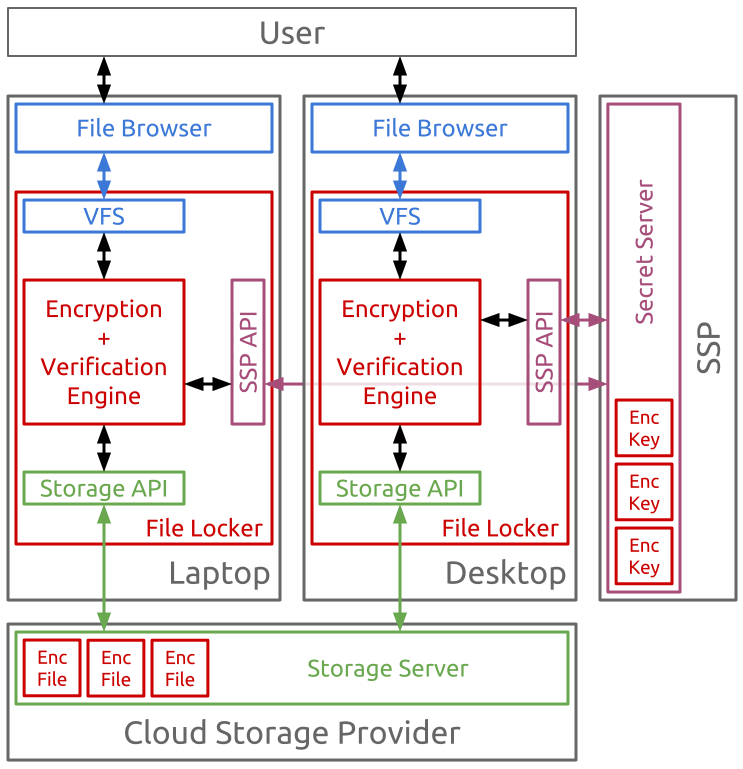
\includegraphics[height=200px]{./figs/out/App-FileLocker.pdf}
  \caption{SSaaS-Backed Cloud File Locker System}
  \label{fig:apps-filestore}
\end{figure}

Building on the original motivating example in this proposal,
i.e. using Dropbox without trusting Dropbox, we can construct an
SSaaS-backed cloud sync and storage
client. Figure~\ref{fig:apps-filestore} illustrates this
application. As in the general storage case, this application involves
applying client-side encryption/decryption (e.g. using
AES~\cite{nist2001}) and authentication/verification (e.g. using
CMAC~\cite{dworkin2005}) on every read and write to a third-party
backed data store. The third-party data store holds only encrypted and
authenticated data, ensuring that the third party need not be granted
Access (\emph{R}-type) and Manipulation (\emph{W}-type) capabilities.

In order to ensure that users can still share data with other users
and sync it across devices, all required encryption and authentication
keys are stored with one or more SSPs. When a user wishes to sync data
to a new device, they grant said device access to the necessary keys
via their SSP's management interface. The new device can then download
the encrypted files from the minimally trusted storage provider and
decrypt/verify them using the keys provided by the SSP. Device
authentication can be provided via certificates, shared-secrets
(e.g. passwords), or contextual information. When a user wishes to
share data with another user, they grant the new user access to
encrypted data via the storage provider's normal sharing
mechanisms. They then also grant the new user access to the necessary
keys via the SSP's management mechanisms. The user can now download
the data from the storage provider and decrypt and verify it with the
keys from the SSP. As in the multi-device sync case, authentication
may be performed via a variety of mechanisms, allowing the data owner
to select the authentication primitives best suited for a given
situation.

This type of application overcomes the traditional deficiencies of
secure cloud-based data storage. It minimizes trust in the third party
storage provider by only granting them access to encrypted and
authenticated data. It also maintains support for the multi-device and
multi-user use cases traditionally associated with cloud-backed data
storage. The SSaaS model allows users to enhance their privacy and
security by reducing exposure to third parties without incurring
additional usability burdens or denying access to desirable features.

\subsection{Server Data Encryption}

Beyond consumer-oriented SSaaS-backed encryption systems, there's
strong case for using SSaaS-backed encryption systems for
datacenter-based servers. Leveraging virtual (as well as physical)
servers hosted in cloud data centers is an extremely popular
deployment method. Unfortunately, as mentioned in
Chapter~\ref{chap:challenges}, the administrator's lack of physical
access to such servers makes it difficult to utilize privacy-enhancing
technologies like Full Disk Encryption (FDE) or file-system level
encryption. In the FDE case, users are generally required to provide
some form of decryption pass-phrase or physical dongle at boot time in
order to securely bootstrap the system. Similarly, even in the
file-system level encryption case, encryption systems generally
require some form of interactive mechanism to provide the necessary
security pass-phrase bootstrapping the system. Since administrators
generally lack easy physical access to datacenter-based servers as
well as interactive presence on headless servers using traditional
encryption systems with most cloud servers remains difficult, if not
impossible.

These deficiencies can largely be resolved by relying on SSaaS-backed
encryption systems - either full disk or file-system oriented. Using
SSaaS, a user would configure each server to store their file
encryption and verification keys with an SSP (or SSPs), configuring
each server to request the keys from the SSP at boot or on access to
an encrypted file. Non-interactive authentication could be provided
using contextual security techniques~\cite{hulsebosch2005} (e.g. do
you expect a server to be rebooted at a certain time of day each day?)
to allow for such encryption systems to operate largely
autonomously. In more sensitive situations, the SSP's access control
system could even keep the user in the loop as in the traditional case
by asking the user to provide a pass-phrase or decryption approval via
text message or similar out-of-band real time communication method
each time key access is required.

Such systems would allow users to store sensitive data on servers
while minimizing the degree of trust they must place in third-party
data center hosts. Such servers would store all data in an encrypted
form, ensuring that a physical search of the server or other
interference from the data center host would not be easy. Encrypted
data could be decrypted on-demand, making it very difficult for the
data center host to access it without employing high degrees of
subterfuge. Even in cases where the data center host does manage to
leverage their control of the underlying physical systems to trick an
SSP into providing decryption keys, the SSP would still be able to log
and audit the event -- making it extremely difficult for a data center
host to access secure user data in an undetectable manner.

Possible implementations of server-based encryption efforts are
discussed further in Chapter~\ref{chap:planned}. Such implementations
would provide a mechanism to significantly decrease the amount of
trust developers (and by proxy, their users) must place in the
providers of hosted server infrastructure without significantly
raising the cost or overhead of leveraging such infrastructure.

\subsection{Mobile Device Encryption}

Beyond of the world of hosted storage systems, the SSaaS model
provides benefit for the protection of local storage as well. Mobile
devices such as phones tables and laptops store huge quantities of
personal information. Yet these devices are more prone to theft and
loss then traditional computing systems such as desktops and
servers. The encryption and protection of such devices is thus a high
priority when working to increase the privacy and security of many
users.

Traditional device encryption systems have become prevalent in Android
and iOS-base mobile devices~\cite{ars-android-encrypt,
  ars-ios-encrypt}. Such systems are useful for ensuring that
device-stored data can not be accessed when devices are shutdown or
(when properly designed) locked, but they do little to protect data
when the phone is (are has recently been) in use. Furthermore, the
encryption keys for such systems are stored locally (often via an HSM)
and are generally only protected with a short pin or pass-phrase.

Such encryption systems could be converted to an SSaaS model where the
keys are stored with one or more SSPs, providing a number of benefits
over local key storage. First, since keys are stored off-device in an
SSaaS-backed encryption system, it's easy to revoke access to the keys
remotely in the event that a device is lost or stolen, ensuring that
an attacker can not guess a user's PIN and access their data. Second,
such a systems could be used to protect individual pieces of data
separately vs the current practice of unlocking all data when the
device starts up. In doing so, it would be possible for a user to set
per-app access control rules with their SSP, effectively reducing the
trust the user must place in the third-party apps they install on
their devices. Users could leverage the SSaaS model to audit all app
data access and limit apps to accessing only the data they are
expected to need. Finally, an SSaaS system could provide more flexible
access control semantics's on mobile devices then the standard
Everything/Nothing access model common today. For example, as SSaaS
system could be setup to provide keys to one set of data to User A
while providing keys to a separate set of data for User B --
effectively protecting per-user data on multi-user devices. Similarly,
an SSaaS system could be configured to provide access overrides in
specific situations -- e.g. allowing an authorized secondary user to
access the device and the data it stores in the event that the primary
user becomes incapacitated (e.g. similar to the functionality provided
by Google's Inactive Account Manager~\cite{atlantic-google-iam}, but
with cryptographic guarantees).

\subsection{Personal Data Repository}

\begin{figure}[t]
  \centering
  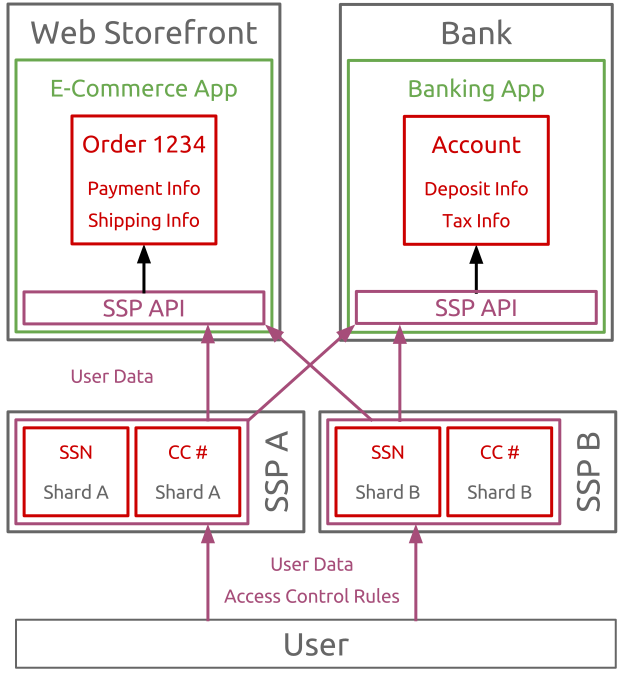
\includegraphics[height=200px]{./figs/out/App-DataRepo.pdf}
  \caption{SSaaS-Backed Personal Data Repo}
  \label{fig:apps-datarepo}
\end{figure}

Moving past encrypted storage applications, we could also leverage the
SSaaS model to create a dedicated repository of personal user info
(e.g SSN, address, etc). Entering personal user data on various
websites is a common user requirement for placing orders, creating
accounts, etc. This practice is undesirable for several reason. First,
it is highly burdensome: users are continually forced to reenter the
same info again and again and must ensure they keep it up to date
across multiple sites. Second, it distributes a lot of sensitive user
data across a large number of actors in a manner that is very
difficult for a user to track or control. Instead, I propose that a
user shard their data across several SSPs and then point websites that
require it directly at the SSPs themselves. The user can then specify
Access Control rules with each SSP allowing specific websites access
to the minimum data they require.

Not only does this approach provide a central repository where the
user can enter personal data and keep it up to date (e.g. when
moving), but it also allows the user to limit each site's access to
only certain data and provides an audit trail for the user to track
exactly which sites have accessed which
data. Figure~\ref{fig:apps-datarepo} illustrates such a use case. In
this case, as opposed to the previous applications, we'll be storing
sensitive user data directly with our SSPs. As such it will be
important to shard the data across multiple SSPs in order to minimize
the trust we must place in each individual SSP.

Such applications could go a long ways toward minimizing the amount of
sensitive personal data we have stored with large number of third
parties in favor of concentrating it on only a handful of SSPs. Doing
so both reduces the trust we must place with any single SSP and
ensures the data is being stored with parties better incentivized to
protect it (see the discussion in Section~\ref{chap:ssaas:trust}).

\section{Communication}

\begin{figure}[t]
  \centering
  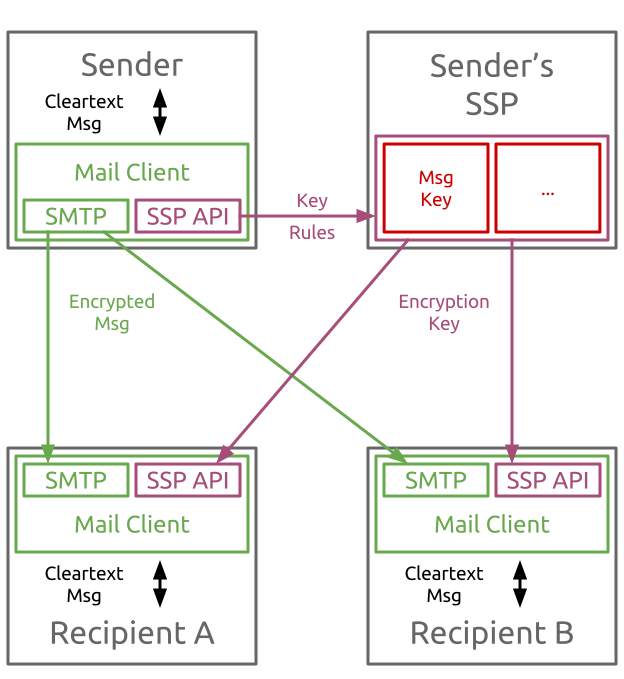
\includegraphics[height=200px]{./figs/out/App-SecureEmail.pdf}
  \caption{SSaaS-Backed Secure Email System}
  \label{fig:apps-secureemail}
\end{figure}

The applications of SSaaS are not limited to data storage. Another
potential area of application involves secure communication between
two or more parties. Such secure messaging systems are in growing
demand, especially after the Snowden revelations related to US
Government monitoring of email and associated digital communication
systems~\cite{gellman-muscular, greenwald-collect,
  greenwald-prism}. While solutions like GnuPG~\cite{gnupg} exist to
allow users to secure the contents of their mail, their complexity
tends to limit their use to a small subset of advanced
users~\cite{green-challenge, whitten1999}. The secure communication
paradigm could be simplified through the use of SSPs and the SSaaS
model.

Figure~\ref{fig:apps-secureemail} illustrates a potential SSaaS secure
communication use case. In this application, a user's mail client
would encrypt the contents and subject of a user's email prior to
sending it with a locally-generated single-use symmetric encryption
key. The client would then upload this key to the user's SSP where the
user would specify that their intended recipients should have read
access to the key. The user could then send the encrypted mail. When
received, the recipient's mail client would request the required key
from the sender's SSP, providing appropriate credentials to prove
their identity in the process, decrypt, and read the email. This
system would be capable of supporting multi-recipient systems like
newsgroups and would also allow the user to grant read access to
additional users after the fact (e.g. should the recipient wish to
forward the email to an additional trusted party), both capabilities
that traditional public-key based email encryption systems struggle to
support. Similar applications could be designed for real-time
communication such as chat.

As in previous cases, third party trust can be minimized by sharding
keys across multiple SSPs. Furthermore, such systems could guarantee
some degree of forward secrecy by having the SSP automatically expire
and delete keys after a certain period of time -- something that
traditional email encryption systems struggle to support. Such designs
have the potential to raise the default level of security inherent in
mass digital communication without significantly inconveniencing
users.

\section{Authentication}

SSaaS also has applications in the authentication realm. Cryptographic
authentication systems (i.e. certificate-based authentication) are
considered to be some of the most secure forms of digital
authentication -- far better then more commonly deployed shared-secret
(i.e. password) authentication systems. Where as shared secret
authentication merely relies on both the user and the verifier
(e.g. server) knowing a common secret such as a pass-phrase,
certificate-based authentication systems rely on a user to be able to
cryptographically prove they posses the private key corresponding to a
specific public key. Such systems have a range of applications, from
authentication on websites to authentication on servers and
workstations. In the latter case, SSH~\cite{ylonen1996} is one of the
more common remote-access protocols for Unix-like computing systems
such as Linux and OSX. SSH uses keys on both the server side, where
they provide server verification and encryption for connecting
clients, as well as on the client side, where they can (optionally) be
used to authenticate users instead of passwords. SSH is thus a useful
example to demonstrate the potential benefits of the SSaaS model to
authentication systems. SSaaS can provide usability and security
benefits to SSH on both the client and server.

\subsection{SSH Agent Key Management}

\begin{figure}[t]
  \centering
  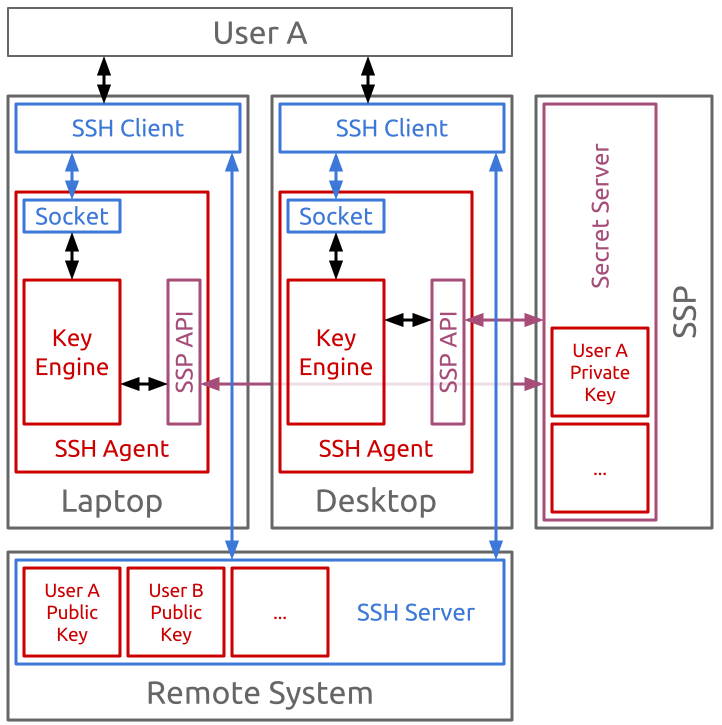
\includegraphics[height=200px]{./figs/out/App-SSHAgent.pdf}
  \caption{SSaaS-Backed SSH Agent}
  \label{fig:app-sshagent}
\end{figure}

The management of private cryptographic keys has long been a challenge
for users. To help mitigate this challenge the systems community has
developed the concept of an ``agent'' program. Agent programs sit
between the user and an authentication system, providing the required
cryptographic keys on the user's behalf to the authentication system
when required~\cite{cox2002}. Agents are commonly used with popular
computing utilities like SSH~\cite{ylonen1996} and
GnuPG~\cite{gnupg}. Unfortunately, existing agent solutions are
designed for legacy usage models: single-device, non-portable desktop
environments. They do not provide a mechanism for managing private
keys across multiple devices, securing keys if the associated device
is lost or stolen, or managing keys for a large group of users across
an organization.

The locality and management challenges associated with traditional
cryptographic agent programs can be overcome by using an SSaaS-backed
agent. Figure~\ref{fig:app-sshagent} shows the basic design for an
SSaaS-backed SSH-agent. Instead of storing private keys locally, such
an agent would defer private key storage to one or more dedicated
SSPs. When the agent requires the user's private keys, it requests
them from the SSP. Thus, the user and any associated agent programs
are able to securely access the necessary private keys from multiple
devices (e.g. laptop, desktop, tablet). Furthermore, if the user ever
loses one of their devices, they can greatly reduce the risk of
exposing any of their private keys by revoking the lost device's
access to the off-site SSaaS data (e.g. similar to~\cite{geambasu2011}
and~\cite{tang2012}). Such a system would also allow large
organizations to manage SSH or other cryptographic keys for all their
users from a centralized SSaaS management applications.

Divorcing private SSH key storage from local devices opens up a range
of use case possibilities, increases security by keeping keys off of
frequently lost or stolen portable devices, and relieves the user of
the usability overhead required to manually manage their private keys.

\subsection{SSH Server Key Management}

\begin{figure}[t]
  \centering
  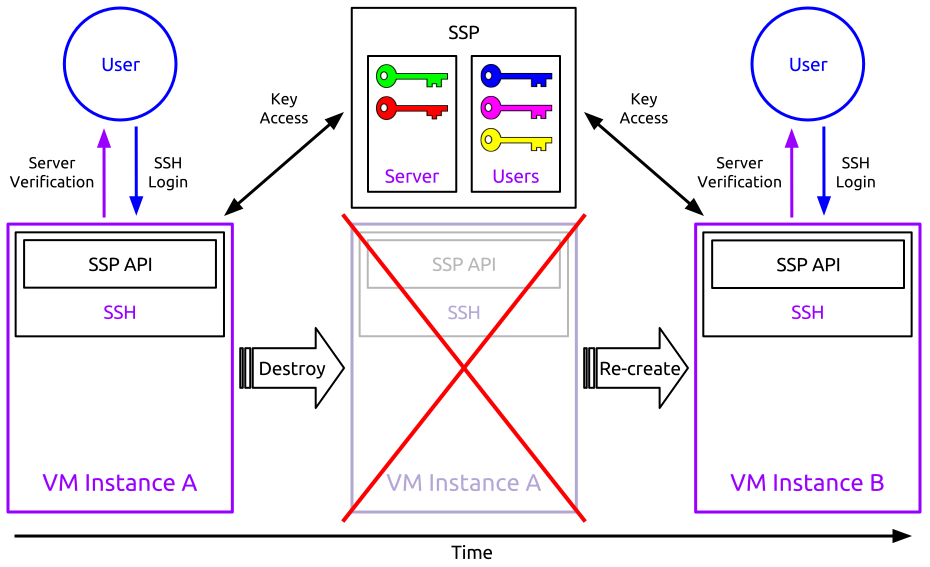
\includegraphics[height=200px]{./figs/out/App-SSHServer.pdf}
  \caption{SSaaS-Backed SSH Server Key Management}
  \label{fig:apps-sshserver}
\end{figure}

Similarly, the SSaaS model can provided benefits when applied to the
server side of SSH. An SSH server must manage both a server key pair,
used to prove the server's identity to a user and to bootstrap the
negotiation of a session key, as well as a list of user public keys
for any users granted server access. Unfortunately, managing both sets
of keys manually poses a number of challenges. Integrating server-side
SSH key management with an SSaaS system can help alleviate these
challenges.

In the server key case, the ephemeral nature of modern IaaS-based
systems causes issues with locally manged keys. For instance, what the
user perceives of as a single server may actually be multiple
load-balanced servers, or may be a single virtual server that is
destroyed and recreated frequently in response to upgrades and changes
in demand. In either case, it's important that the user be able to
properly authenticate that the server they are accessing is in fact
the correct server and not malicious man-in-the-middle
attacker. Unlike SSL, however, SSH does not rely on a central
certificate authority structure for the verification of keys. Instead
it uses a ``trust on first use'' model that fingerprints a server key
the first time the user connects and then assumes that this key will
remain associated with a given server address indefinitely. If an
ephemeral cloud server generates a new server SSH key each time it's
recreated, or if multiple logically equivalent, load-balanced servers
all have different SSH keys, a user will be unable to verify that the
server is equivalent to the one they originally accessed. This issue
could be overcome by storing the SSH verification keys for a server
with one or more SSPs as shown in
Figure~\ref{fig:apps-sshserver}. Then, when a server is recreated, or
when a single logical server is balanced between multiple instances,
it still has access to the same SSH keys originally in use, ensuring
that previous users can properly authenticate the server as valid.

The server's list of authorized user keys poses similar
challenges. These lists contain the public keys of all users
authorized to access a given server. Maintaining such lists across
large numbers of servers, and ensuring they stay up to date even as
individual server instances are added, removed, and upgraded is
challenging. Failing to properly manage such lists can either lead to
legitimate users being locked out of systems, or worse, allowing
illegitimate users (e.g. a previous employee) to access systems they
should not. Indeed, such misconfiguration errors are one of the
leading causes of security failures today~\cite{bishop1996,
  kerravala2002}. Centralizing the management of such authorized keys
lists with an SSP allows administrators to manage and audit server
access across a wide collection of infrastructure from a single
place. Such a solution is the SSaaS equivalent of cloud user
management solutions such as JumpCloud~\cite{jumpcloud}. But unlike
existing services, an SSaaS-backed SSH user management system avoids
trusting any single third party by leveraging the key-sharding
possibilities available in an SSaaS ecosystem.

Both of these setups illustrate the benefits an SSaaS system can
provide to common authentication and user management problems in cloud
servers. In many ways, SSaaS represents a more secure variant of
traditional configuration management solutions such as
Chef~\cite{chef} or Puppet~\cite{puppet}. But unlike such solutions,
the SSaaS model is deigned with the security and privacy of the
configuration data it stores as a first principle, not a secondary
concern.

\section{Dedicated Crypto Processor}

\begin{figure}[t]
  \centering
  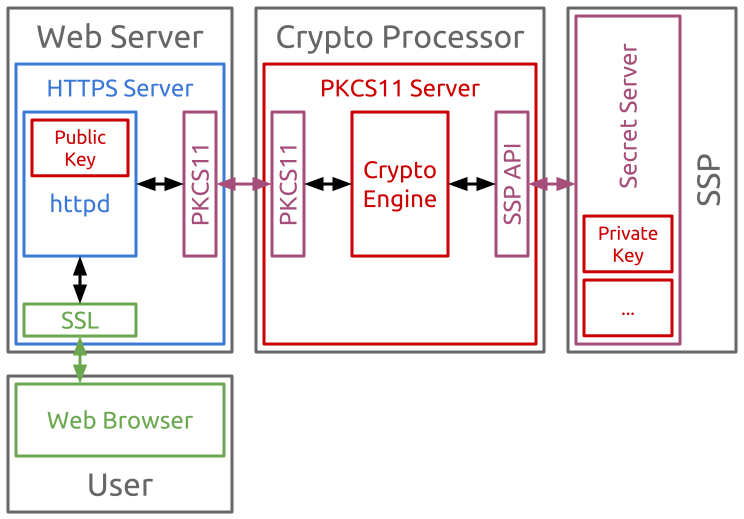
\includegraphics[height=200px]{./figs/out/App-PKCS11.pdf}
  \caption{SSaaS-Backed Dedicated Crypto Processor}
  \label{fig:app-pkcs11}
\end{figure}

The recent Heartbleed bug~\cite{heartbleed} exposed one of the main
risks of embedding cryptographic secret storage within the
applications requiring access to these secrets: when applications
break, they also risk exposing access to the private keys stored in
the same memory segments. The Heartbleed fallout has forced everyone
to reevaluate whether or not giving public-facing services direct
access to cryptographic keys is a good idea. There has long existed an
alternative: using a hardware security module (HSM) to perform
dedicated crypto processing and key storage on behalf of other
services. Such systems ensure that cryptographic keys are never
exposed outside of the secure hardware module. Programs communicate
with the HSM via a standard protocol like
PKCS\#11~\cite{pcks11-standard}. In such systems, an application sends
the HSM clear-text data to encrypt and gets back the encrypted
ciphertext in return. Unfortunately, most existing HSM solutions don't
scale to the performance levels required by high-volume services. This
has led some to suggest moving to a software-based ``HSM''
model~\cite{lorier-pkcs11}. Such softHSM systems would still ensure
cryptographic keys remain stored in separate isolated memory spaces
while also out-performing traditional HSM systems.

A software-based dedicated crypto processing system is an ideal use
case an SSaaS-backed system. Figure~\ref{fig:app-pkcs11} shows the
potential design of such a system. Here, a Secret Storage Provider
supplies the back-end key storage for a dedicated crypto processing
server which performs cryptographic operations (e.g. SSL encryption
and authentication) on behalf of a web-server. In this setup, the
web-server never accesses any private cryptographic keys directly,
mitigating one of the major risks Heartbleed exposed. Furthermore, the
logically centralized nature of an SSaaS SSP allows dedicated crypto
processing servers to scale horizontally (e.g. multiple load-balancing
instances) as demand requires: storing all keys via one or more SSPs
allows new crypto processing instances to immediately access these
keys without the need to utilize ad-hoc key-syncing or configuration
management interfaces. Furthermore, The SSP's auditing functionality
ensures that you always know which keys have been accessed by which
systems, placing hard bounds on what an attacker may or may not have
had access too: a luxury that Heartbleed-prone servers did not have.

Such a design combines the benefits of a dedicated crypto-processor
with the third-party trust limiting nature of the SSaaS model. This
combination allows for high speed cryptographic processing without
placing a high degree of trust in any single system or party.

%%  LocalWords:  SSaaS CMAC SSPs SSP's SSP FDE iOS Repo Snowden IaaS
%%  LocalWords:  JumpCloud Heartbleed PKCS softHSM
